\documentclass[12pt]{article}
\usepackage{amsthm,amssymb,amsfonts,amsmath,amstext,systeme}
\usepackage{graphicx,float}
\usepackage{tabularx}

\marginparwidth 0pt
\oddsidemargin -1.2 truecm
\evensidemargin  0pt 
\marginparsep 0pt
\topmargin -2.2truecm
\linespread{1}
\textheight 25.8 truecm
\textwidth 18.5 truecm
\newenvironment{remark}{\noindent{\bf Remark }}{\vspace{0mm}}
\newenvironment{remarks}{\noindent{\bf Remarks }}{\vspace{0mm}}
\newenvironment{question}{\noindent{\bf Question }}{\vspace{0mm}}
\newenvironment{questions}{\noindent{\bf Questions }}{\vspace{0mm}}
\newenvironment{note}{\noindent{\bf Note }}{\vspace{0mm}}
\newenvironment{summary}{\noindent{\bf Summary }}{\vspace{0mm}}
\newenvironment{back}{\noindent{\bf Background}}{\vspace{0mm}}
\newenvironment{conclude}{\noindent{\bf Conclusion}}{\vspace{0mm}}
\newenvironment{concludes}{\noindent{\bf Conclusions}}{\vspace{0mm}}
\newenvironment{dill}{\noindent{\bf Description of Dill's model}}{\vspace{0mm}}
\newenvironment{maths}{\noindent{\bf Mathematics needed}}{\vspace{0mm}}
\newenvironment{inst}{\noindent{\bf Instructions}}{\vspace{0mm}}
\newenvironment{notes}{\noindent{\bf Notes }}{\vspace{0mm}}
\newenvironment{theorem}{\noindent{\bf Theorem }}{\vspace{0mm}}
\newenvironment{example}{\noindent{\bf Example }}{\vspace{0mm}}
\newenvironment{examples}{\noindent{\bf Examples }}{\vspace{0mm}}
\newenvironment{topics}{\noindent{\bf Topics}}{\vspace{0mm}}
\newenvironment{outcomes}{\noindent{\bf Expected Learning Outcomes}}{\vspace{0mm}}
\newenvironment{lemma}{\noindent{\bf Lemma }}{\vspace{0mm}}
\newenvironment{solution}{\noindent{\it Solution}}{\vspace{2mm}}
\newcommand{\ds}{\displaystyle}
\newcommand{\un}{\underline}
\newcommand{\bs}{\boldsymbol}

\begin{document}

\baselineskip 18 pt
\begin{center}
	{\large \bf HKDSE MATH M2 Practice Paper}\\
	\vspace{2 mm}

\end{center}
\vspace{0.05cm}

\begin{enumerate}
	\item \textbf{HKDSE Math M2 Practice Paper Q1}\\
	Find the coefficient of $x^5$ in the expansion of $(2-x)^9$. \\(4 marks)


	\item \textbf{HKDSE Math M2 Practice Paper Q2}\\
	Consider the following system of linear equation in $x$, $y$, $z$
	$$\left\{\begin{matrix}
		x & - & 7y & + & 7z & = & 0\\
		x & - & ky & + & 3z & = & 0\\
		2x & + & y & + & kz & = & 0\\
	\end{matrix}\right.\text{ , where }k\text{ is a real number.}$$
	If the system has non-trival solutions, find the two possible values of $k$. \\(4 marks)


	\item \textbf{HKDSE Math M2 Practice Paper Q3}\\
	Prove by mathematical induction that $4^n+15n - 1$ is divisible by 9 for all positive integers $n$. \\(5 marks)
		

	\item \textbf{HKDSE Math M2 Practice Paper Q4}
	\begin{enumerate}
		\item [(a)]Let $x = \tan{\theta}$, show that $\displaystyle\frac{2x}{1+x^2} = \sin{2\theta}$. 
		\item [(b)]Using (a), find the greatest value of $\displaystyle\frac{(1+x)^2}{1+x^2}$, where $x$ is real.
	\end{enumerate}
	(5 marks)

	\item \textbf{HKDSE Math M2 Practice Paper Q5}
	\begin{enumerate}
		\item [(a)]It is given that $\cos{(x+1)} + \cos{(x-1)} = k\cos{x}$ for any real $x$. Find the value of $k$. 
		\item [(b)]Without using a calculator, find the value of $\begin{vmatrix}
			\cos{1} & \cos{2} & \cos{3}\\
			\cos{4} & \cos{5} & \cos{6}\\
			\cos{7} & \cos{8} & \cos{9}\\
		\end{vmatrix}$.
	\end{enumerate}
	(6 marks)

	\item \textbf{HKDSE Math M2 Practice Paper Q6}\\
	Find $\displaystyle\frac{d}{dx}\left(\frac{1}{x}\right)$ from first principles. \\(4 marks)

	\item \textbf{HKDSE Math M2 Practice Paper Q7}\\
	Let $f(x) = e^x(\sin{x} + \cos{x})$. 
	\begin{enumerate}
		\item[(a)]Find $f'(x)$ and $f''(x)$. 
		\item[(b)]Find the value of $x$ such that $f''(x) - f'(x) + f(x) = 0$ for $0 \leq x \leq \pi$.
	\end{enumerate}
	(5 marks)

	\item \textbf{HKDSE Math M2 Practice Paper Q8}
	\begin{enumerate}
		\item [(a)]Using integration by substitution, find $\displaystyle\int\frac{dx}{\sqrt{4-x^2}}$. 
		\item [(b)]Using integration by parts, find $\displaystyle\int\ln{x}\,dx$.
	\end{enumerate}
	(5 marks)

	\item \textbf{HKDSE Math M2 Practice Paper Q9}\\
	Find the equations of the two tangents to the curve $x^2 - xy -2y^2 -1 =0$ which are parallel to the straight line $y = 2x+1$. \\(6 marks)

	\item \textbf{HKDSE Math M2 Practice Paper Q10}
	\begin{enumerate}
		\item [(a)]Find $\displaystyle\int xe^{-x^2} \,dx$. 
		\item [(b)]In Figure 1, the shaded region is bounded by the curves $y = \displaystyle\frac{x^2}{2}$ and $y = e^{-x^2}$, where $1 \leq x \leq 2$. Find the volume of the solid generated by revolving the shaded region about the $y$-axis.
		\begin{figure}[H]
			\centering
			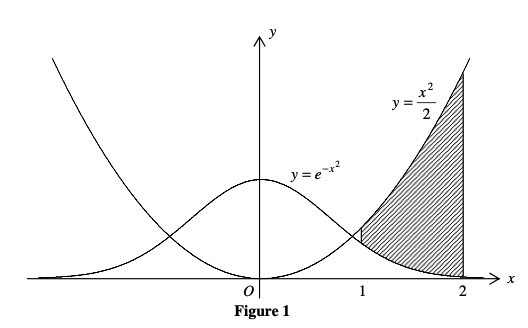
\includegraphics[width = .5\linewidth]{PPFigure1}
		\end{figure}
	\end{enumerate}
	(6 marks)

	\item \textbf{HKDSE Math M2 Practice Paper Q11}\\
	Let $A = \begin{pmatrix}
		\alpha + \beta & -\alpha\beta \\
		1 & 0 \\
	\end{pmatrix}$ where $\alpha$ and $\beta$ are distinct real numbers. Let $I$ be the $2\times2$ identity matrix.  
	\begin{enumerate}
		\item [(a)]Show that $A^2 = (\alpha +\beta)A - \alpha\beta I$. \\(2 marks)
		\item [(b)]Using (a), or otherwise, show that $(A - \alpha I)^2 = (\beta - \alpha)(A - \alpha I)$ and $(A - \beta I)^2 = (\alpha - \beta)(A - \beta I)$. \\(3 marks)
		\item [(c)]Let $X = s(A-\alpha I)$ and $Y = t(A-\beta I)$ where $s$ and $t$ are real numbers. \\
		Suppose $A = X + Y$.
		\begin{enumerate}
			\item [(i)]Find $s$ and $t$ in terms of $\alpha$ and $\beta$.
			\item [(ii)]For any positive integer $n$, prove that \\
			$X^n = \displaystyle\frac{\beta^n}{\beta - \alpha} (A - \alpha I)$ and $Y^n = \displaystyle\frac{\alpha^n}{\alpha - \beta}(A - \beta I)$.
			\item [(iii)]For any positive integer $n$, express $A^n$ in the form of $pA + qI$, where $p$ and $q$ are real numbers.  
			[Note: It is known that for any $2\times2 $ matrices $H$ and $K$,\\
			if $HK = KH = \begin{pmatrix}
				0&0\\0&0\\
			\end{pmatrix}$, then $(H+K)^n = H^n + K^n$ for any positive integer $n$.]
		\end{enumerate}
		(9 marks)
	\end{enumerate}

	\item \textbf{HKDSE Math M2 Practice Paper Q12}\\
	Let $\overrightarrow{OA} = \textbf{i}$, $\overrightarrow{OB} = \textbf{j}$ and $\overrightarrow{OC} = \textbf{i} + \textbf{j} + \textbf{k}$ (see Figure 2). Let $M$ and $N$ be points on the straight lines $AB$ and $OC$ respectively such that $AM:MB = a:(1-a)$ and $ON:NC = b:(1-b)$, where $0 < a < 1$ and $0 < b < 1$. Suppose that $MN$ is perpendicular to both $AB$ and $OC$.
	\begin{figure}[H]
		\centering
		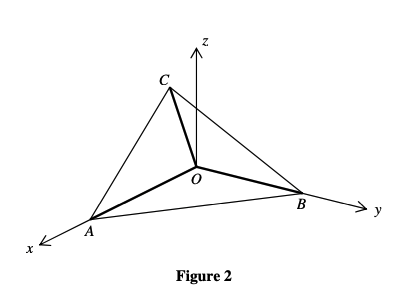
\includegraphics[width = .5\linewidth]{PPFigure2}
	\end{figure}
	\begin{enumerate}
		\item [(a)]
		\begin{enumerate}
			\item [(i)]Show that $\overrightarrow{MN} = (a+b-1)\textbf{i} +(b-a) \textbf{j} +b \textbf{k}$. 
			\item [(ii)]Find the values of $a$ and $b$.
			\item [(iii)]Find the shortest distance between straight lines $AB$ and $OC$.
		\end{enumerate}
		(8 marks)
		\item [(b)]
		\begin{enumerate}
			\item [(i)]Find $\overrightarrow{AB}\times\overrightarrow{AC}$. 
			\item [(ii)]Let $G$ be the projection of $O$ on the plane $ABC$, find the coordinates of the intersecting point of the two straight lines $OG$ and $MN$.
		\end{enumerate}
		(5 marks)
  	\end{enumerate}

	\item \textbf{HKDSE Math M2 Practice Paper Q13}
	\begin{enumerate}
		\item[(a)]Let $f(x)$ be an odd function for $-p \leq x \leq p$, where $p$ is a positive constant.\\
		Prove that $\displaystyle\int_0^{2p} f(x-p)\,dx = 0$.\\
		Hence evaluate $\displaystyle\int_0^{2p} [f(x-p)+q]\,dx $, where $q$ is a constant. \\(4 marks)
		\item[(b)]Prove that $\displaystyle\frac{\sqrt{3} + \tan{\left(x - \displaystyle\frac{\pi}{6}\right)}}{\sqrt{3} - \tan{\left(x - \displaystyle\frac{\pi}{6}\right)}} = \frac{1+\sqrt{3}\tan{x}}{2}$. \\(2 marks)
		\item[(c)]Using (a) and (b), or otherwise, evaluate $\displaystyle\int_0^{\frac{\pi}{3}} \ln{(1 + \sqrt{3}\tan{x})} \,dx$. \\(4 marks)
	\end{enumerate}

	\item \textbf{HKDSE Math M2 Practice Paper Q14}
	\begin{enumerate}
		\item[(a)]In Figure 3, the shaded region enclosed by the circle $x^2 + y^2 = 25$, the $x$-axis and the straight line $y = h$ (where $0 \leq h \leq 5$) is revolved about the $y$-axis. Show that the volume of the solid of revolution is $\left(25h - \displaystyle\frac{h^3}{3}\right)\pi$. \\(2 marks)
		\begin{figure}[H]
			\centering
			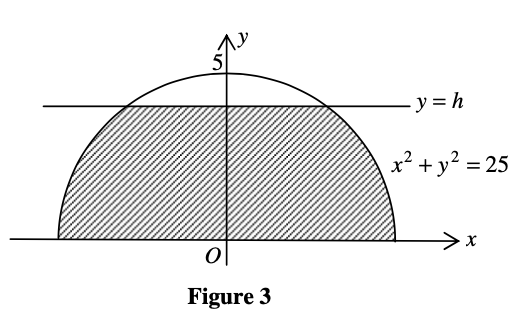
\includegraphics[width = .5\linewidth]{PPFigure3}
		\end{figure}		
		\item[(b)]In Figure 4, an empty coffee cup consists of two portions. The lower portion is in the shape of the solid described in (a) with height 4 cm. The upper portion is a frustum of a circular cone. The height of the frustum is 8 cm. The radius of the top of the cup is 6 cm. Hot coffee is poured into the cup to a depth $h$ cm at a rate of 8 cm$^3$s$^{-1}$, where $0 \leq h \leq 12$. Let $V$ cm$^3$ be the volume of coffee in the cup. 
		\begin{figure}[H]
			\centering
			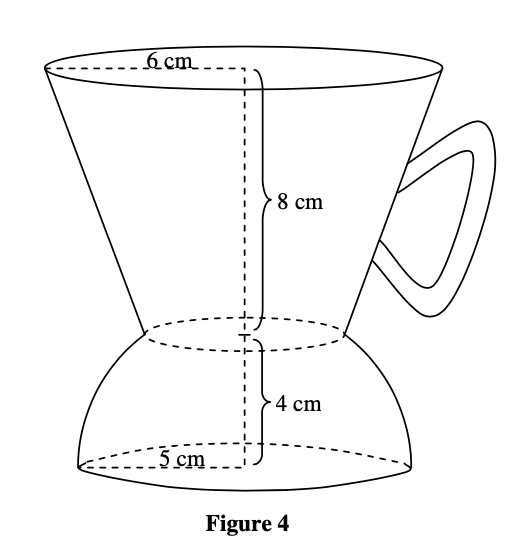
\includegraphics[width = .5\linewidth]{PPFigure4}
		\end{figure}
		\begin{enumerate}
			\item [(i)]Find the rate of increase of the depth of coffee when the depth is 3 cm.
			\item [(ii)]Show that $V = \displaystyle\frac{164\pi}{3} + \frac{3\pi}{64}(h+4)^3$ for $4\leq h \leq 12$. 
			\item [(iii)]After the cup is fully filled, suddenly it cracks at the bottom. The coffee leaks at a rate of 2 cm$^3$s$^{-1}$. Find the rate of decrease of the depth of coffee after 15 seconds of leaking, giving your answer correct to 3 significant figures.
		\end{enumerate}
		(11 marks)
	\end{enumerate}
\end{enumerate}


\end{document}